\columnbreak
\section*{\LARGE Modelling synaptic lifetime distributions with Kesten processes}

In an experimental study by \textcite{Loewenstein2015} chronic in-vivo two-photon imaging revealed that the lifetime dynamics of spines in the neocortex follow a power law. Motivated by results from detailed network simulations, we here consider a simple stochastic model based on the Kesten process in order to analyze how different properties of a cortical network might affect the lifetime distributions of synaptic spines.

\subsection*{Model}

Kesten process have been used before \cite{Statman2014} to describe spine size dynamics. In this model, a given spine size $X_n$ at time step $n$ is updated as
%
\begin{align}
  X_{n+1} = a_n X_n + b_n. \label{eq:kesten}
\end{align}
%
In this further simplified form we take $a_n$ to be a fixed value of $a_n=0.9987$, while the additive change is drawn from a normal distribution, $b_n \sim \mathcal{N}(\mu_b, \sigma_b^2)$. Then, to model synapse growth and pruning processes, we consider a population of $N$ synapses. Each synapse has a random time $T_{\mathrm{init}}$, uniformly distributed in $[0,T_{\text{max}}]$, at which it is initialized with size $X_0$. The synapse size $X_t$ then evolves according to \eqref{eq:kesten}.

The lifetime of the synapse is the number of time steps from $T_{\text{init}}$ until for the first time $X_t < X_{\mathrm{prune}}$. In this case the synapse gets pruned and a new synapse with size $X_0$ is inserted in the network (Fig~\ref{fig:km}). In the case that $X_t$ doesn't fall below $X_{\mathrm{prune}}$ until $T_{\text{max}}$, the lifetime is recorded as $T=T_{\text{max}}-T_{\text{init}}$. At the end of the simulation the sizes $X_{T_{\text{max}}}$ are recorded for all $N$ synapses.

\begin{center}\vspace{1cm}
  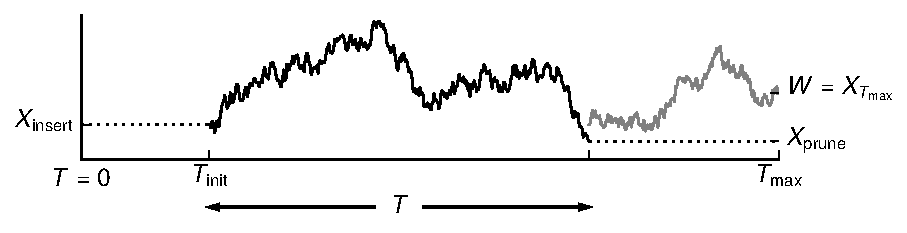
\includegraphics[width=0.85\columnwidth]{%
    figures/abstract_fig.pdf}
  %% /home/fh/sci/lab/syn_lt/kesten_model/note_x/km_ca_rts_dd/img/abstract_fig.png}
  \captionof{figure}{Adapted Kesten simulation model allows the tracking of lifetimes and size distributions}
  \label{fig:km}
\end{center}\vspace{1cm}


\subsection*{Results}

We simulated \SI{5e5} synapses evolving as Kesten processes and recorded lifetime and weight distributions. For unbiased additive change ($\mu_b =0$), a power law like distribution of synaptic lifetimes emerges (Fig~\ref{fig:lifetimes}A). The distribution of spine sizes $X_{T_{\text{max}}}$ resembles a log-normal distribution, as one might expect from findings on the synaptic weight distributions in cortical circuits \cite{Song2005}.

\vspace{1.2cm}
\begin{overpic}[width=\columnwidth]%
  % 110, 133
  {figures/lifetimes_weights.png}
  %\put(32,\ylin){anisotropic}
  \put(1,28){\normalfont \textbf{A}}
  \put(52,28){\normalfont \textbf{B}}
\end{overpic}
\captionof{figure}[format=hang,indention=1cm]{Dynamical properties of network connectivity modelled by Kesten processes. \textbf{A} Lifetime distribution of synapses created at time step $T_{\text{init}}$ uniformly distributed in $[0, T_{\text{max}}]$. \textbf{B} Distribution of spine sizes $X_{T_{\text{max}}}$ at time step $X_{T_{\text{max}}}$ (grey) and log-normal fit (red). Parameters for both: $a=0.9987$, $\mu_b=0$, $\sigma_b^2=0.22$, $X_{\text{insert}}=0.1$, $X_{\text{prune}}=0.01$. \label{fig:lifetimes}}

\vspace{3cm}

%% \begin{center}\vspace{1cm}
%%   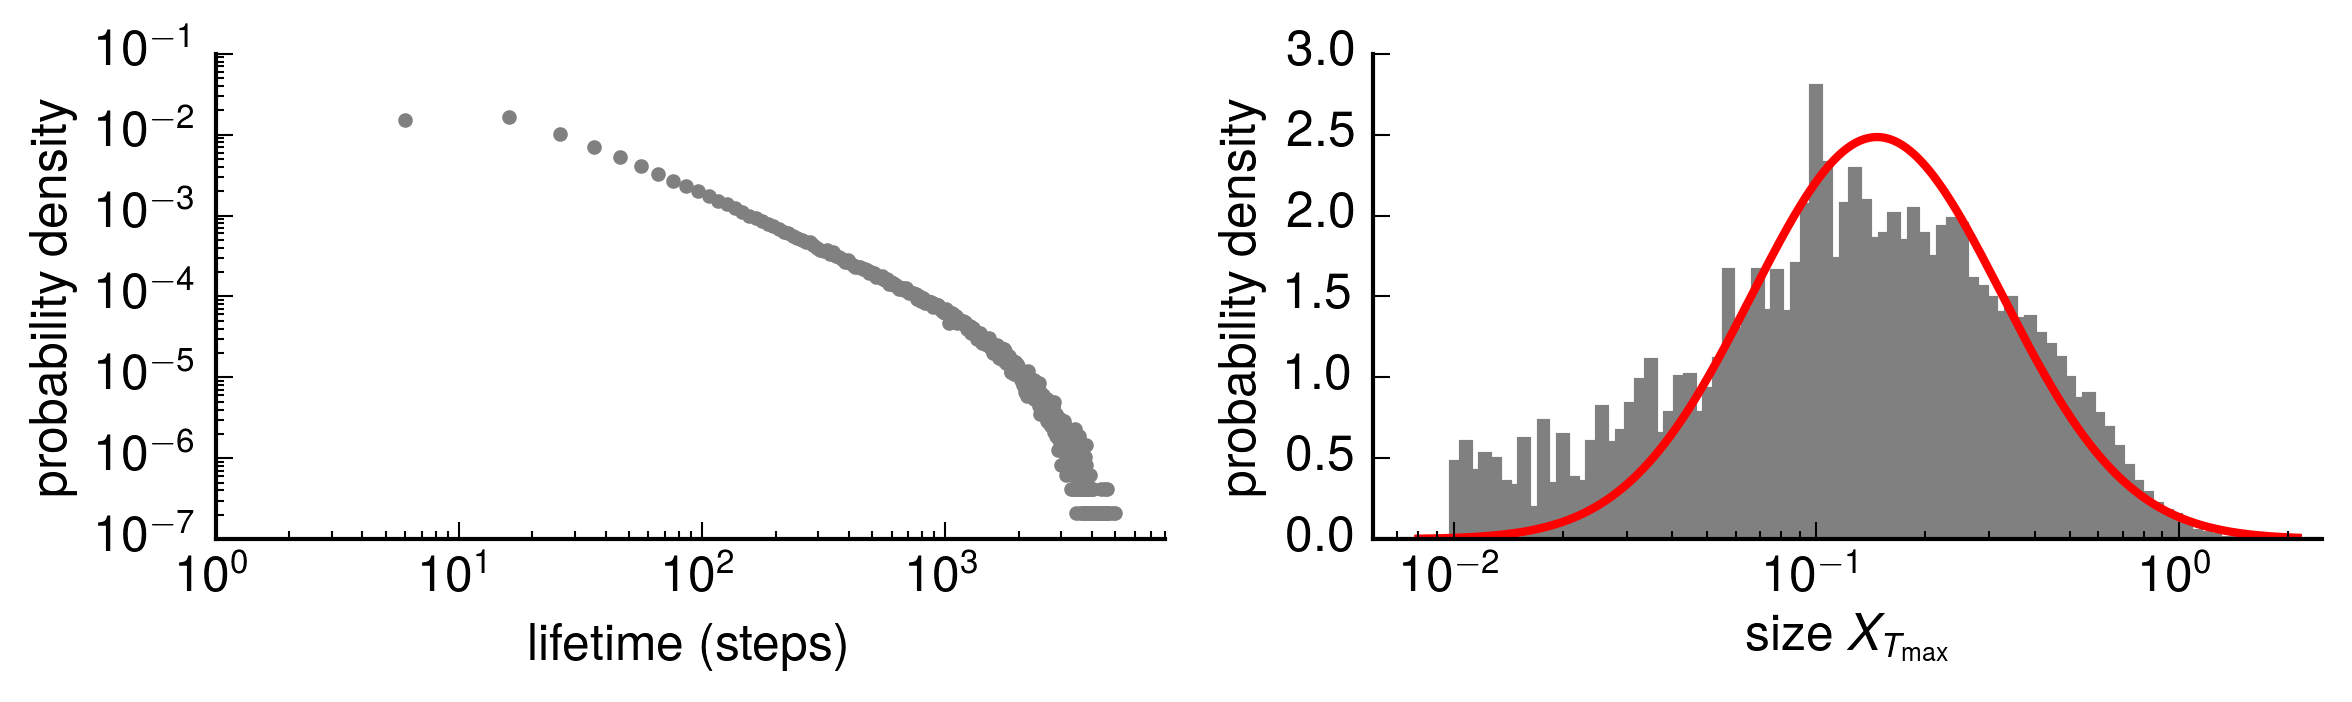
\includegraphics[width=\columnwidth]{%
%%     %% /home/fh/sci/lab/syn_lt/kesten_model/note_x/km_ca_rts_dd/img/lifetimes_weights.png}
%%     figures/lifetimes_weights.png}

%%   \captionof{figure}{}
%%   \label{fig:lifetimes}
%% \end{center}\vspace{1cm}

Next, we explored how different parameters in the model affect the lifetime and spine size distributions. We found that varying $\sigma_b^2$ has little effect on the distributions. Interestingly, however, the bias in the additive change affect both distributions significantly. As one might expect . This result also 

\begin{center}\vspace{1cm}
  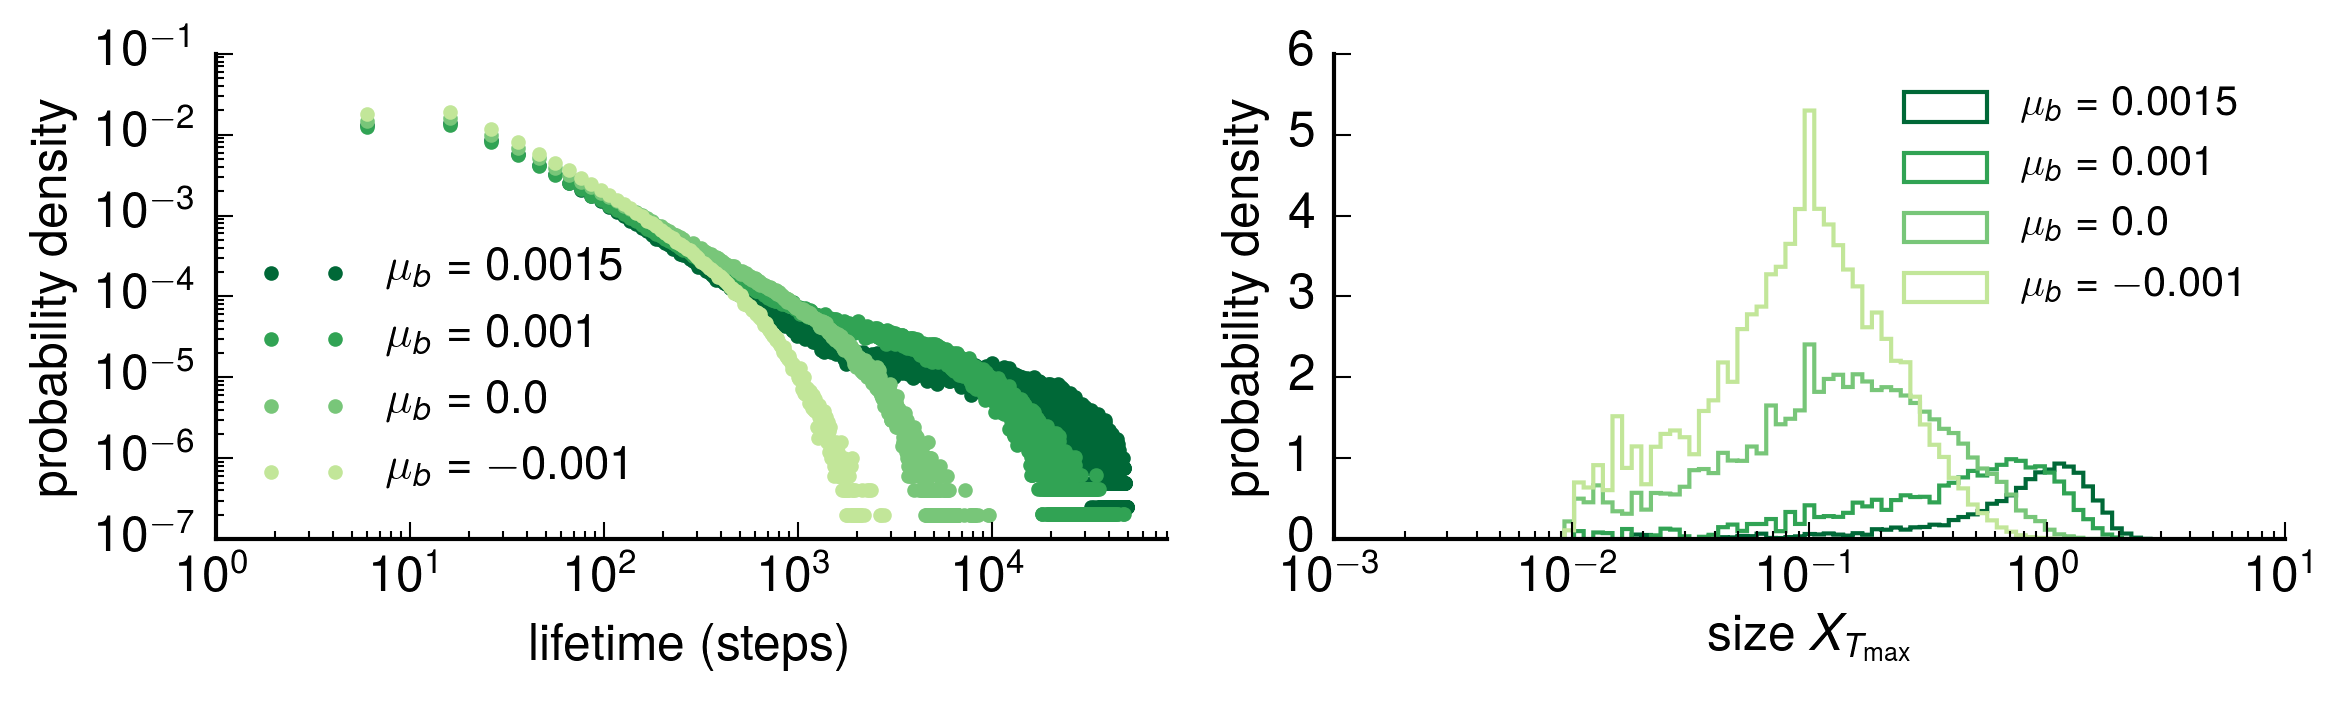
\includegraphics[width=\columnwidth]{%
%% /home/fh/sci/lab/syn_lt/kesten_model/note_x/km_ca_rts_dd/img/lifetimes_weights_mub_compare.png}
   figures/lifetimes_weights_mub_compare.png}
  \captionof{figure}{}
\end{center}\vspace{1cm}





